

\section{Background and Motivation}

Every option trade has a buyer and seller side. For a plethora of problems in option research, it’s also crucial to determine the party that initiated the transaction. Applications include the study of option demand \autocite[][]{garleanuDemandBasedOptionPricing2009}, of informational content in option trading \autocites[][]{huDoesOptionTrading2014}[][]{panInformationOptionVolume2006}[][]{caoInformationalContentOption2005}, of order flow \autocite[][]{muravyevOrderFlowExpected2016}, or of trading costs \autocite[][]{muravyevOptionsTradingCosts2020}. 

Despite the clear importance for empirical research, the true initiator of the trade is frequently absent in datasets and is inferred using trade classification rules \autocite[][]{easleyOptionVolumeStock1998}. In consequence, the correctness of empirical studies hinges on the algorithm's ability to accurately identify the trade initiator.

Popular heuristic to sign trades are the tick test \autocite[][]{hasbrouckTradesQuotesInventories1988}, quote rule \autocite[][]{harrisDayEndTransactionPrice1989}, and hybrids thereof such as the \gls{LR} algorithm \autocite[][]{leeInferringTradeDirection1991}. These rules have initially been proposed and tested in the stock market. For option markets, the works of \textcites[][]{savickasInferringDirectionOption2003}[][]{grauerOptionTradeClassification2022} raise concerns about the transferability of trade signing rules due to deteriorating classification accuracies and systematic misclassifications. The latter is crucial, as non-random misclassifications bias the dependent research \autocites[][]{odders-whiteOccurrenceConsequencesInaccurate2000}[][]{theissenTestAccuracyLee2001}.

A second, growing body of research \autocites{blazejewskiLocalNonParametricModel2005}{rosenthalModelingTradeDirection2012}{ronenMachineLearningTrade2022} advances trade classification performance through \gls{ML}. The scope of current works is yet focused on the stock market and the \textit{superficial} setting, where supervised models are trained on fully-labeled trades. Then again, labeled trades are difficult to obtain, whereas unlabeled trades are abundant.

The goal of our empirical study is to investigate if a \gls{ML}-based classifier can improve upon the accuracy of state-of-the-art approaches in option trade classification.

\section{Contributions}

Our contributions are threefold: 
\begin{enumerate}[label=(\roman*),noitemsep]
\item By employing \glspl{GBRT} and Transformers we establish a new state-of-the-art in option trade classification. We outperform existing approaches by \SI{3.73}{\percent}~-~\SI{6.51}{\percent} in accuracy on a large sample of \gls{ISE} trades. Relative to the ubiquitous \gls{LR} algorithm, improvements are up to \SI{17.02}{\percent}. 
The model's efficacy is demonstrated for alternative trading venues, in sub-samples, and in an application study.
\item Our work is the first to consider trade classification also in the semi-supervised scenario, in which trades are only partially labeled. Our best models classify \SI{74.55}{\percent} (+ 6.94) of all trades correctly.
\item Through a feature importance analysis based on Shapley values, we can consistently attribute performance gains of rule-based and \gls{ML}-based classifiers to feature groups. We show that both paradigms share common features, but \gls{ML}-based approaches more effectively exploit the data.
\end{enumerate}

\section{Data}

We perform the empirical analysis on two large-scale datasets of option trades recorded at the \gls{ISE} and \gls{CBOE}. Our sample construction follows \textcite[][]{grauerOptionTradeClassification2022}, which fosters comparability between both works. 

Training and validation are performed exclusively on \gls{ISE} trades. After a time-based train-validation-test split, required by the \gls{ML} estimators, we are left with a test set spanning from Nov. 2015 -- May 2017 at the \gls{ISE}. \gls{CBOE} trades between Nov. 2015 -- Oct. 2017 are used as a second test set. Each test set contains between 9.8 Mio. --  12.8 Mio. labeled option trades. An additional unlabeled, training set of \gls{ISE} trades executed between Oct. 2012 -- Oct. 2013 is reserved for learning in the semi-supervised setting.

To establish a common ground with rule-based classification, we distinguish three feature sets with increasing data requirements and employ minimal feature engineering. The first set is based on the data requirements of tick/quote-based algorithms, the second of hybrid algorithms with additional dependencies on trade size data, and the third feature set includes option characteristics, like the option's $\Delta$ or the underlying. 

\section{Methodology}

We model trade classification using \glspl{GBRT} \autocites[][]{friedmanGreedyFunctionApproximation2001}, a wide tree-based ensemble, and the FT-Transformer \autocite{gorishniyRevisitingDeepLearning2021}, a Transformer-based neural network architecture. We select these approaches for their state-of-the-art performance in tabular modeling \autocites[][]{gorishniyRevisitingDeepLearning2021}[][]{grinsztajnWhyTreebasedModels2022} and their extendability to learn on partially-labeled trades. Additionally, Transformers offer \textit{some} model interpretability through the Attention mechanism. An advantage we exploit later to derive insights into the classification process of Transformers.

As stated earlier, our goal is to extend \gls{ML} classifiers for the semi-supervised setting to make use of the abundant, unlabeled trade data. We couple gradient-boosting with self-training \autocite{yarowskyUnsupervisedWordSense1995}, whereby confident predictions of unlabeled trades are iteratively added into the training set as pseudo-labels. A new classifier is then retrained on labeled and pseudo-labeled trades. Likewise, the Transformer is pre-trained on unlabeled trades with the replaced token detection objective \autocite{clarkElectraPretrainingText2020} and later finetuned on labeled training instances. Conceptually, the network is tasked to detect randomly replaced tokens or features of transactions. Both techniques are aimed at improving generalization performance.

Classical trade classification rules are implemented as a rule-based classifier allowing us to construct arbitrary candidates for benchmarking and support richer evaluation of feature importances.\footnote{Our implementation is publicaly available under \url{https://pypi.org/project/tclf/}.}

For a fair comparison, we run an exhaustive Bayesian search, to find a suitable hyperparameter configuration for each of our models. Classical rules have no hyperparameters per se. Akin to tuning the \gls{ML} classifiers on the validation set, we select candidate rules for the classical benchmarks based on their validation performance. This is most rigorous while preventing overfitting the test set. The so-selected benchmarks come from a recent paper of \textcite{grauerOptionTradeClassification2022}, which we subsequently refer to as \gls{GSU} method (small/large).\footnote{All of our source code and experiments are publicaly available under \url{https://github.com/KarelZe/thesis/}.}

\section{Results}

Our models establish a new state-of-the-art for trade classification on the \gls{ISE} and \gls{CBOE} dataset, as shown in \cref{tab:results-supervised-ise-cboe}. For \gls{ISE} trades, Transformers achieve an accuracy of \SI{63.78}{\percent} when trained on trade and quoted prices as well as \SI{72.58}{\percent} when trained on additional quoted sizes, improving over current best of \textcite[][]{grauerOptionTradeClassification2022} by \SI{3.73}{\percent} and \SI{4.97}{\percent}. Similarly, \glspl{GBRT} reach accuracies between \SI{63.67}{\percent} and \SI{72.34}{\percent}. We observe performance improvements up to \SI{6.51}{\percent} for \glspl{GBRT} and \SI{6.31}{\percent} for Transformers when models have access to option characteristics. Relative to the ubiquitous tick test, quote rule, and \gls{LR} algorithm, improvements are \SI{23.88}{\percent}, \SI{17.11}{\percent}, and \SI{17.02}{\percent}. Both architectures generalize well on \gls{CBOE} data, with even stronger improvements between \SI{5.26}{\percent} and \SI{7.86}{\percent} over the benchmark depending on the model and feature set. 

In the semi-supervised setting, as shown in \cref{tab:results-semi-supervised-ise-cboe}, Transformers on \gls{ISE} dataset profit from pre-training on unlabeled trades with accuracies up to \SI{74.55}{\percent}, but the performance gains slightly diminish on the \gls{CBOE} test set. Vice versa, we observe no benefits from semi-supervised training of \glspl{GBRT}.

We derive from exhaustive robustness tests, that performance is stable across multiple subsets. Outperformance is strongest for in-the-money options, options with a long maturity, as well as options traded at the quotes.

For an evaluation of feature importances, that suffices for a cross-model comparison, we use \gls{SAGE} \autocite{covertUnderstandingGlobalFeature2020}. It is a global feature importance measure based on Shapley values and is capable of handling complex feature interactions, such as highly correlated quotes and prices. We estimate \gls{SAGE} values in terms of improvement in zero-one loss per feature set, complementing our accuracy-based evaluation.

As evident from \cref{fig:sage-importances} we find, that all models attain the largest improvement in loss from quoted prices and if provided from the quoted sizes. The contribution of the \gls{NBBO} to performance is roughly equal for all models, suggesting that even simple heuristics effectively exploit the data. For \gls{ML}-based predictors, quotes at the exchange level hold equal importance in classification. This contrasts with \gls{GSU} methods, which rely less on exchange level quotes.  The performance improvements from the trade size and quoted size, are slightly lower for rule-based methods compared to \gls{ML}-based methods. Transformers and \glspl{GBRT} slightly benefit from the addition of option features, i.e., moneyness and time to maturity. 

Regardless of the method used, changes in trade price, central to the tick test, are irrelevant for classification and can even harm performance. This result aligns with earlier studies of \textcites{savickasInferringDirectionOption2003}{grauerOptionTradeClassification2022}.

\section{Disucssion}

Advancements in classical trade classification have been fueled by drawing on more complex decision boundaries, e.g., by fragmenting the spread \autocites{ellisAccuracyTradeClassification2000}{chakrabartyTradeClassificationAlgorithms2007} or by assembling multiple heuristics \autocite{grauerOptionTradeClassification2022}. It is thus likely, that the outperformance of our \gls{ML} estimators is due to the more complex, learned decision boundaries.

The strong results of Transformers sharply contradict those of \textcite[][]{ronenMachineLearningTrade2022}, who benchmark random forests and \glspl{FFN} for trade classification in the equity and bond market and find clear dominance of the tree-based approach. First, unlike \gls{FFN}, the FT-Transformer is tailored to learn on tabular data through being a non-rotationally-invariant learner. Second, our data preprocessing and feature engineering are adapted to the requirements of neural networks. Without these measures, tree-based approaches excel due to their robustness in handling skewed and missing data.

An explanation as to why pre-training improves performance on \gls{ISE} but not \gls{CBOE} trades, may be found in the pre-training data and setup. It is conceivable, that pre-training encodes exchange-specific knowledge, such as trading regimes. Trades used for pre-training are recorded at the \gls{ISE} only and are repeatedly shown to the model. While our pre-training objective is stochastic with different features being masked in each step, past research has shown that repeatedly presenting the same tokens in conjunction with a small-sized pre-training dataset, can degrade performance on the downstream classification task. For instance, \textcite[][]{raffelExploringLimitsTransfer2020} document in the context of language modeling that a high degree of repetition encourages memorization in the transformer, but few repetitions are not harmful.

Self-training with \glspl{GBRT} as a base learner generally performs worse than \glspl{GBRT} trained on labeled trades. With the pseudo labels derived from high-confident predictions, the success of self-training hinges on the reliability of the predicted class probabilities. In an analysis of the \gls{GBRT}, we observe that the validation loss in terms of sample-wise loss stagnates due to a growing number of overconfident but erroneous predictions. It is conceivable, that the increased number of confident yet incorrect predictions, affects the generated pseudo labels. Given these observations, we recommend using \glspl{GBRT} for supervised trade classification only. 

\section{Conclusion}

In conclusion, our study showcases the efficacy of machine learning as a viable alternative to existing trade signing algorithms for classifying option trades, if partially-labeled or labeled trades are available for training. Compared to existing approaches, our classifiers also improve robustness, which together reduces noise and bias in option research dependent on reliable trade initiator estimates.

The out-of-sample results are particularly strong for the pre-trained FT-Transformer, indicating that unsupervised pre-training can encode a generalizable knowledge about exchange trading in the model. An interesting venue for future research is to revisit training Transformers on a larger corpus of unlabeled trades through pre-training objectives and study the effects from \textit{exchange-specific} finetuning.

\begin{table*}
    \centering
    \caption[Accuracies of Supervised Classifiers]{Accuracy of supervised \glspl{GBRT} and Transformers for different feature combinations on the \gls{ISE} and \gls{CBOE} datasets. The improvement is estimated as the absolute change in accuracy between the classifier and the benchmark. For the feature set classic \gls{GSU} (small) is the benchmark and otherwise \gls{GSU} (large). Models are trained on the \gls{ISE} training set. The best classifier per dataset is in \textbf{bold}.}
    \label{tab:results-supervised-ise-cboe}
    \begin{tabular}{@{}llSSSSSS@{}}
        \toprule
                   &             & \multicolumn{2}{c}{\glsentryshort{FS} Classic} & \multicolumn{2}{c}{\glsentryshort{FS} Size} & \multicolumn{2}{c}{\glsentryshort{FS} Option}                                                                 \\ \cmidrule(lr){3-4}\cmidrule(lr){5-6} \cmidrule(lr){7-8}
        Dataset    & Classifier  & {Acc. in \%}                                     & {+/-}                                                 & {Acc. in \%}                                  & {+/-}              & {Acc. in \%}        & {+/-}              \\ \midrule
        \gls{ISE}  & \gls{GBRT}  & 63.668637                                        & 3.620000                                              & 72.343640                                     & 4.730000           & \bfseries 74.120496 & \bfseries 6.510000 \\
                   & Transformer & \bfseries 63.783020                              & \bfseries 3.730000                                    & \bfseries 72.581107                           & \bfseries 4.970000 & 73.921795           & 6.310000           \\ \addlinespace
        \gls{CBOE} & \gls{GBRT}  & 66.002029                                        & 5.260000                                              & 71.951794                                     & 5.430000           & \bfseries 74.375033 & \bfseries 7.860000 \\
                   & Transformer & \bfseries 66.182348                              & \bfseries 5.440000                                    & \bfseries 72.153338                           & \bfseries 5.640000 & 74.278318           & 7.760000           \\ \bottomrule
    \end{tabular}
\end{table*}


\begin{table*}
    \centering
    \caption[Accuracies of Semi-Supervised Classifiers]{Accuracy of semi-supervised \glspl{GBRT} and Transformers for different feature combinations on the \gls{ISE} and \gls{CBOE} datasets. The improvement is estimated as the absolute change in accuracy between the classifier and the benchmark. For the feature set classic \gls{GSU} (small) is the benchmark and otherwise \gls{GSU} (large). Models are trained on the \gls{ISE} training set. The best classifier per dataset is in \textbf{bold}.}
    \label{tab:results-semi-supervised-ise-cboe}
    \begin{tabular}{@{}llSSSSSS@{}}
        \toprule
                   &             & \multicolumn{2}{c}{\glsentryshort{FS} Classic} & \multicolumn{2}{c}{\glsentryshort{FS} Size} & \multicolumn{2}{c}{\glsentryshort{FS} Option}                                                                 \\ \cmidrule(lr){3-4}\cmidrule(lr){5-6} \cmidrule(lr){7-8}
        Dataset    & Classifier  & {Acc. in \%}                                     & {+/-}                                                 & {Acc. in \%}                                  & {+/-}              & {Acc. in \%}        & {+/-}              \\ \midrule
        \gls{ISE}  & \gls{GBRT}  & 63.397514                                        & 3.350000                                              & 72.156489                                     & 4.550000           & 73.536644           & 5.930000           \\
                   & Transformer & \bfseries 64.655751                              & \bfseries 4.600000                                    & \bfseries 72.859054                           & \bfseries 5.250000 & \bfseries 74.551410 & \bfseries 6.940000 \\ \addlinespace
        \gls{CBOE} & \gls{GBRT}  & \bfseries 66.189454                              & \bfseries 5.440000                                    & \bfseries 71.922680                           & \bfseries 5.410000 & 73.953322           & 7.440000           \\
                   & Transformer & 65.668441                                        & 4.920000                                              & 71.783984                                     & 5.270000           & \bfseries 74.095833 & \bfseries 7.580000 \\ \bottomrule
    \end{tabular}
\end{table*}

\begin{figure*}[h]
    \centering
    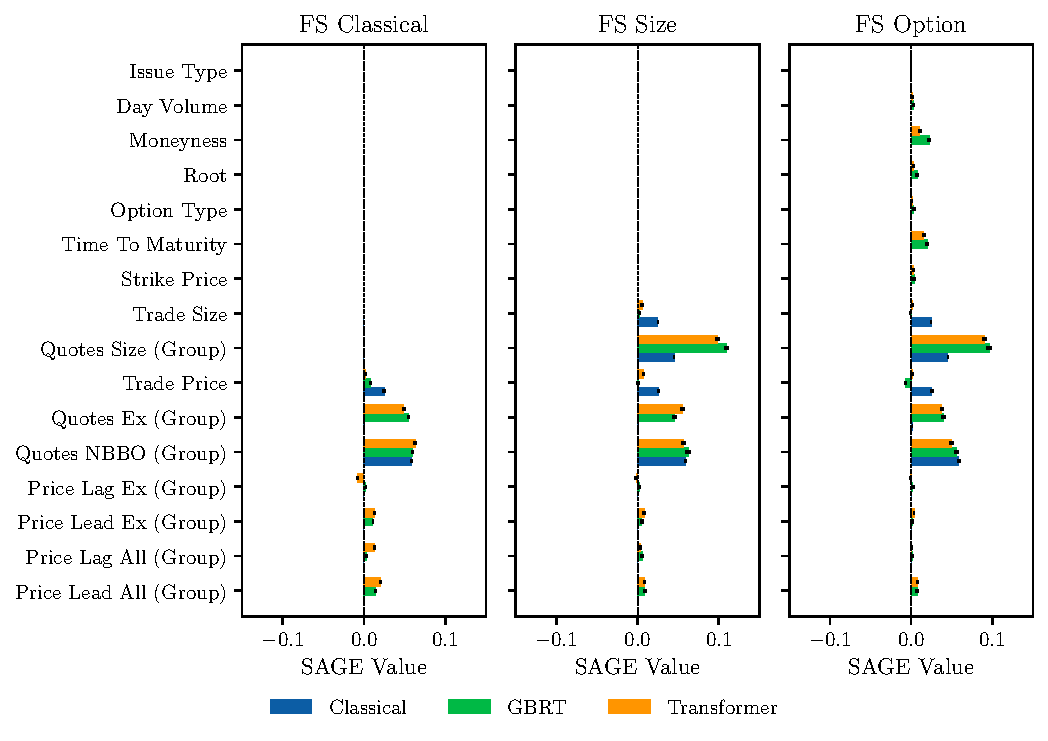
\includegraphics[width=1\textwidth]{sage-importances.pdf}
    \caption[\glsentryshort{SAGE} Feature Importances]{\gls{SAGE} feature importances of rule-based and \gls{ML}-based classifiers. Importances estimated on \gls{ISE} test set with zero-one loss. Bigger feature importances are better. For the feature set classical the \gls{GSU} method (small) is used and otherwise the \gls{GSU} method (large).}
    \label{fig:sage-importances}
\end{figure*}